% !TeX root = guess_who.tex
\documentclass[12pt]{article}
\usepackage[letterpaper, portrait, margin=1in]{geometry}
\usepackage[hidelinks]{hyperref}
\usepackage{setspace}
\usepackage{graphicx}
\usepackage{subcaption}
\usepackage{fancyhdr}
\usepackage[T1]{fontenc}
\usepackage{mathptmx}
\usepackage[backend=biber, style=mla]{biblatex}
\pagestyle{fancy}
\addbibresource{guess_who.bib}    

\fancyhf{} % sets both header and footer to nothing}
\renewcommand{\headrulewidth}{0pt}
\pagenumbering{arabic}
\rhead{Sheehan \thepage} 
\fancypagestyle{1stPage}{
    \fancyhf{}
    \renewcommand{\headrulewidth}{0pt} % removes horizontal header line
    \lhead{\href{mailto:osheehan@andrew.cmu.edu}{Owen M. Sheehan} \\ \href{mailto:stsu@andrew.cmu.edu}{Susan Tsu} \\Basic Design 1 \\12/08/23}
    \rhead{ Sheehan 1}
}

\thispagestyle{1stPage}
\linespread{1.3}
\begin{document}


\vspace*{20pt}
\par Claes Oldenburg was born on January 28, 1929, to Sigrid Elisabeth and Swedish diplomat Gösta Oldenburg in Stockholm.
    The family moved between Stockholm, New York, and Oslo until Claes was 7, when the permanently moved to Chicago.
    Oldenburg studied art, drama, and literature at Yale University, the University of Wisconsin in Madison, and the Art Institute of Chicago. \autocite[1]{bio1}
\par When it comes to Oldenburg's work, he wanted it to be  ``at once crudely provocative, even as it maintained an identity as art'' \autocite[255]{bio2}.
    This sentiment can be seen in what Oldenburg is most famous for, and what I'll be focusing on in this essay, which is his monumnetal sculptures.
    When it comes to the subjects of Oldenburg's (and his usual partner for these sculptures, Coosje van Bruggen's) sculptures, they always focused on ``everyday crap'', with Mark Rosenthal saying, 
    ``[Oldenburg] would certainly agree that the monument is an aspect of the urban landscape, in which human activity predominates, but rather than the usual assortment of subjects --- men in uniform and on horseback --- he wanted a more authentic version of what he called ``city nature'', [which] places an emphasis on ``everyday crap'''' \autocite*[255]{bio2}.
\par For all of Oldenburg's pieces, author Germano Celant says, ``In Oldenburg's terrain, ... the object supplants the human body. It then becomes fraught with perturbations and passions,
    becomes swollen and agitated, rises and falls. Similarly, the human being is transformed into a feeling object. This absurd condition --- objects palpitating like humans, while humans are reduced to objects --- is the crux of Oldenburg's understanding and procedure: the object is given life, while life is annuled in the object'' \autocite*[13]{bio3}.
    This is supported by Oldenburg's own words, with him writing, `` Loving life and movement I am always seeing movement even in the inanimate. I wish simply to create life, which is impossible as I go about it and the result is with my materials the illusion of life, comic or ironic or absurd. It becomes stopped movement or just the opposite of movement. This happens even when my materials are living things, people fex (sic). To freeze in space is of course the very character of art, my method'' \autocite[7]{Oldenburg1}
\par Oldenburg in his later days, focused almost exclusively on monumental sculpture, which is sensibly made out of manufacturing materials such as steel. (see Figure \ref{fig:stake}).
    Whereas, in his earlier days, Claes would make soft sculpture out of foam filled canvas or vinyl. (see Figure \ref{fig:fan}).
\par To me, one of the most striking of Oldenburg and van Bruggen's sculptures is "Trowel I" (fig. \ref{fig:trowel}). It feels, personally, like a perfect example of Oldenburg's work. It shows the juxtaposition common to his monuments. Oldenburg has put a sculpture here that classically ``doesn't fit''.
    It has quite a rigid and manufactured feeling that is in opposition to the natural and flowing trees. However, on the other hand, it doesn't feel violent, even though the framing would make you think that it should be. I'm bad at describing art, but I think you get my point, Oldenburg makes something that, by all means, should feel alien feel somewhat alive and like it belongs, it a weird juxtaposition in my mind.
\par This, to me, that is the sheer delight of Oldenburg's work, that feeling of having something that feels like shouldn't work be masterfully composed in a way that makes it make perfect sense. This points back to what Celant said earlier about how Oldenburg breathes life into banal objects \autocite{bio3}, which I think is a perfectly apt way to put it. On paper, these monuments should feel lifeless and out of place, but, they just don't, which is magical.
\par I know this comes of as a little bit rambly, however, it's hard for me verbalize how I feel and interpret art. I hope my writing somehow  


\newpage

% #region Figures =======================
\begin{figure}[t]
    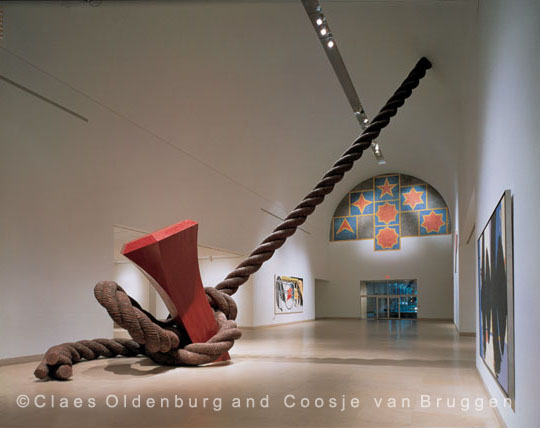
\includegraphics[width=0.5\textwidth,height=0.4\textheight]{stake1.jpg}
    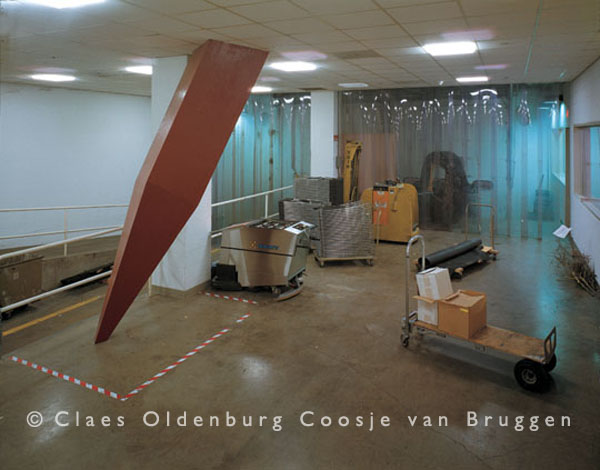
\includegraphics[width=0.5\textwidth,height=0.4\textheight]{stake2.jpeg}
    \caption{Stake Hitch at Dallas Museum of Art \autocite{Pic1}}
    \label{fig:stake}
\end{figure}

\begin{figure}
    \begin{subfigure}{0.5\textwidth}
    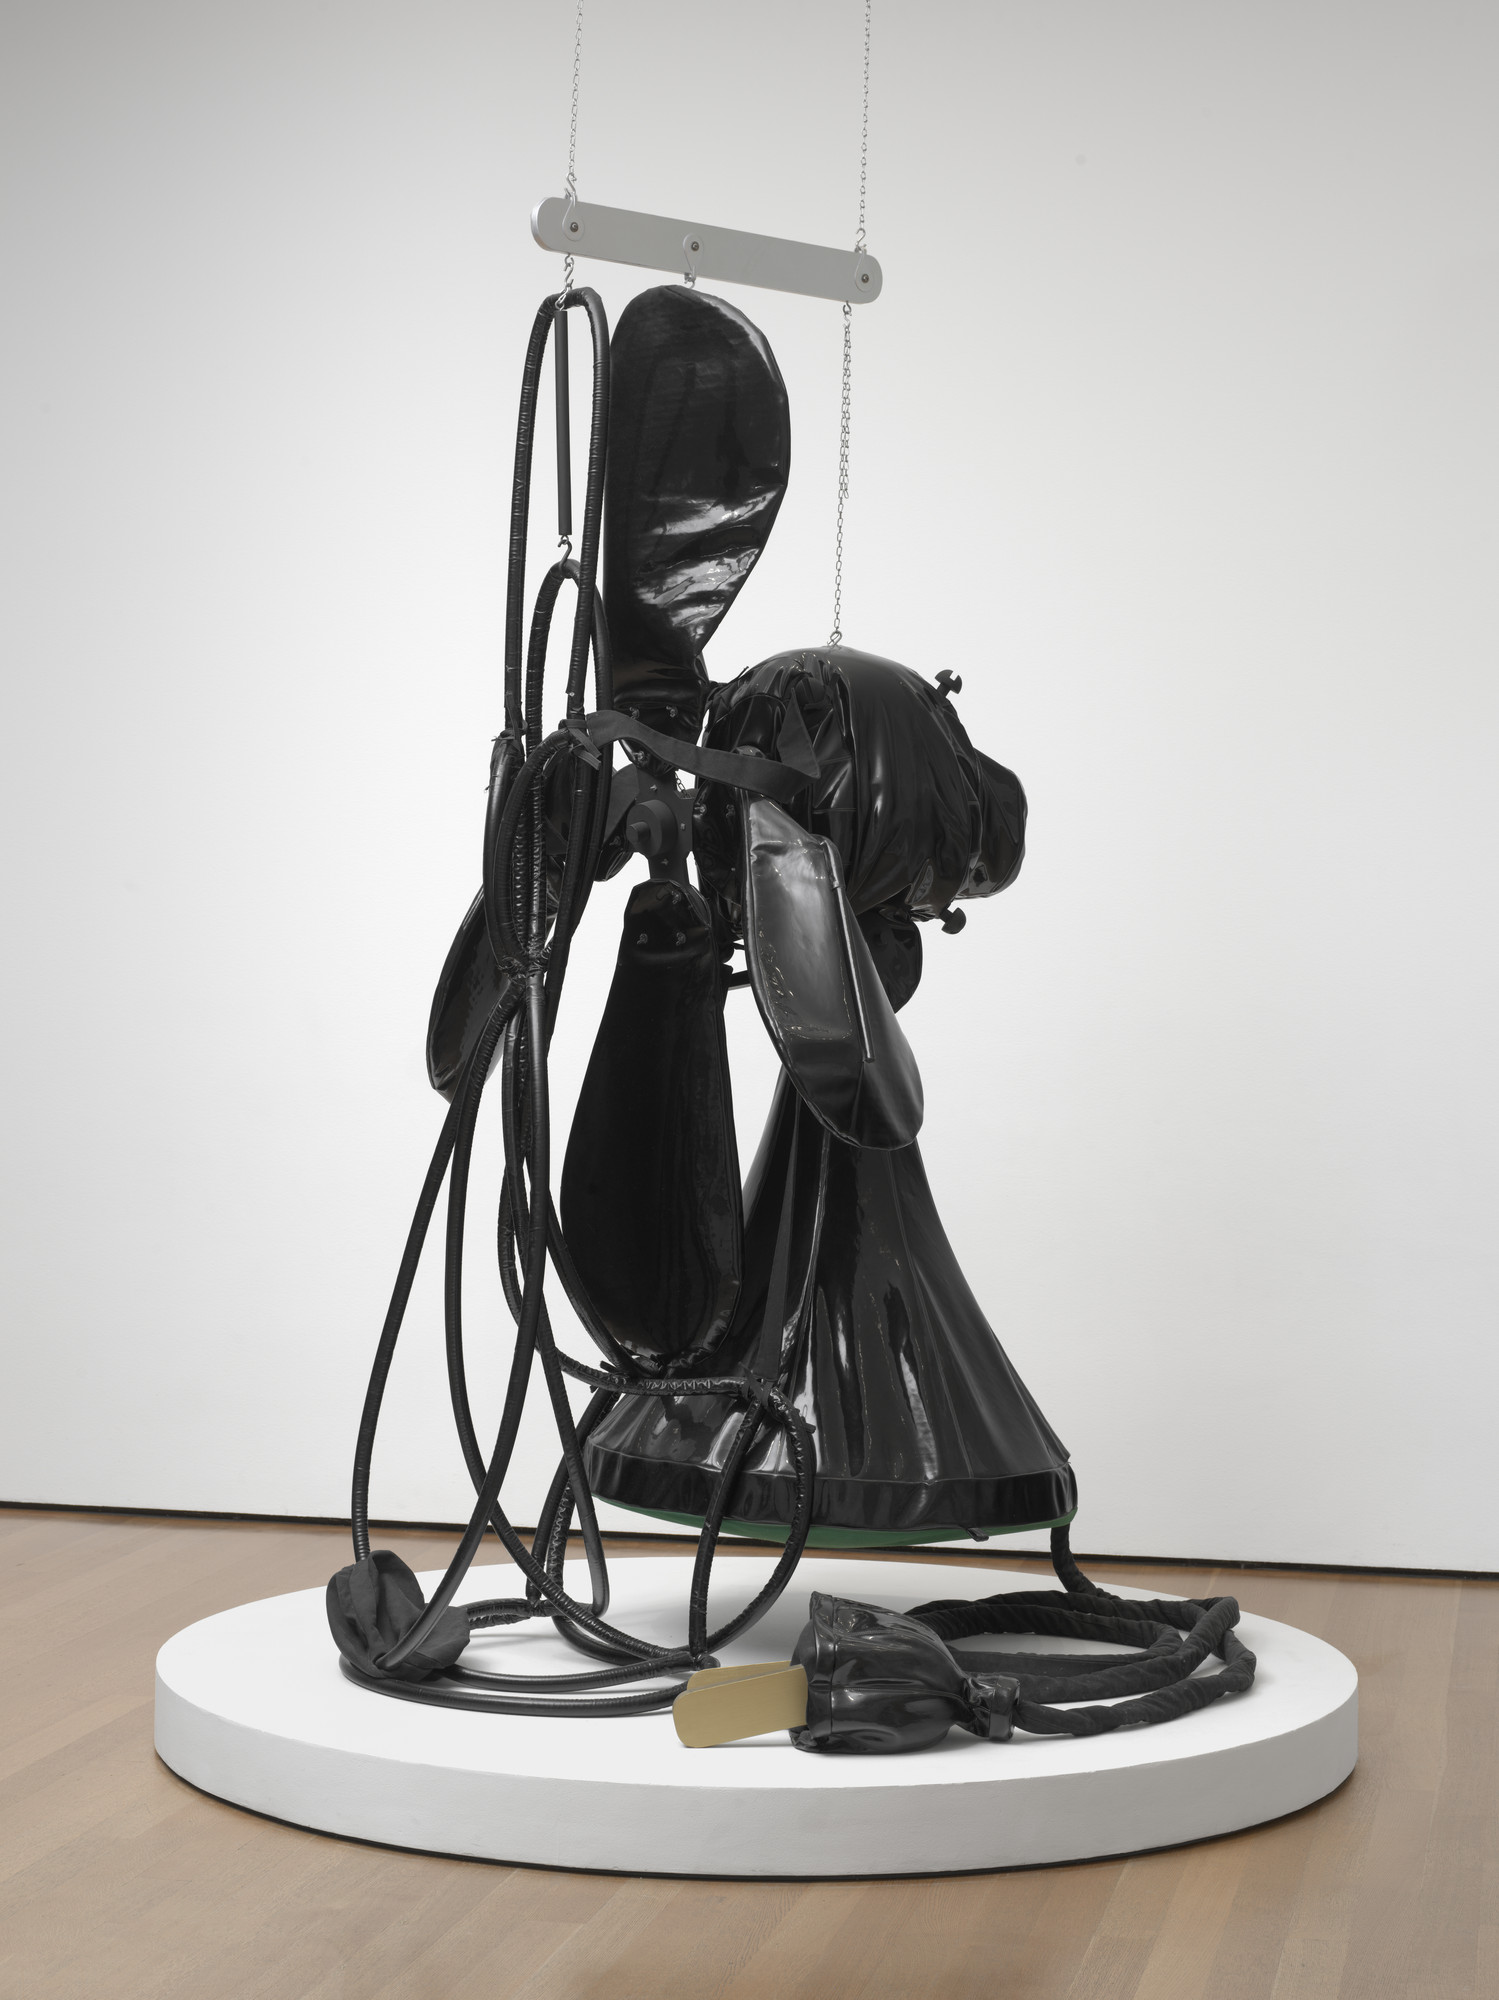
\includegraphics[height=.4\textheight]{fan1.jpeg}
        \centering
        \caption{Giant Soft Fan \autocite{pic2}}
        \label{subim1}
    \end{subfigure}
    \begin{subfigure}{0.5\textwidth}
        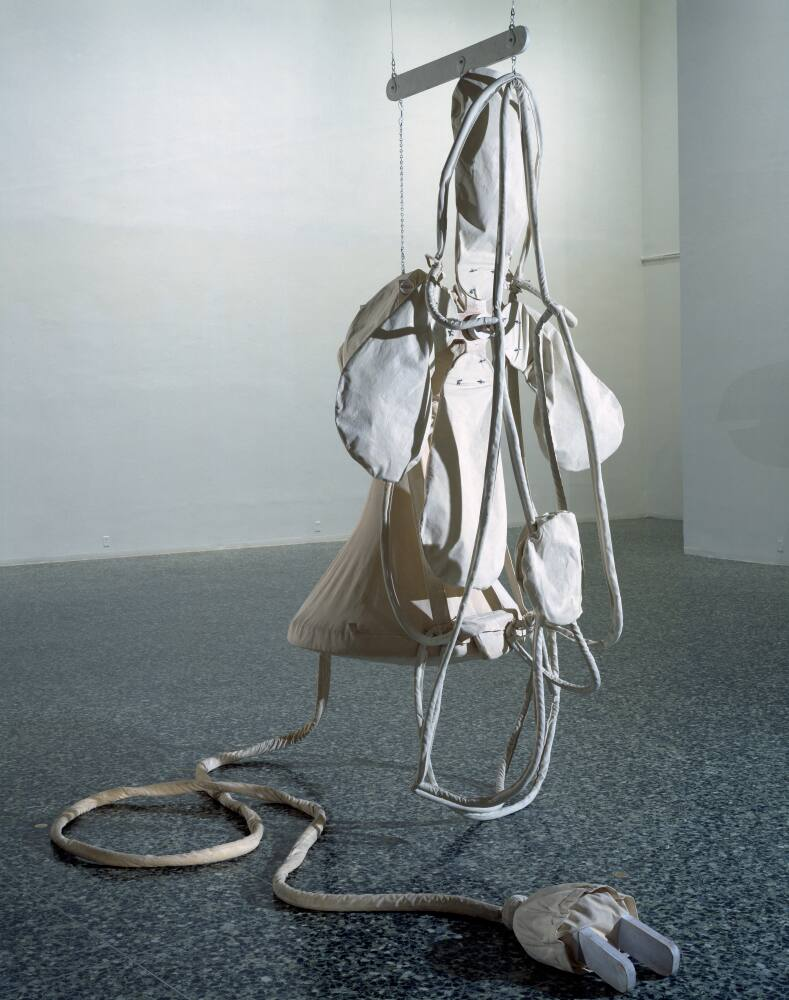
\includegraphics[height=.4\textheight]{fan2.jpeg}
        \centering
        \caption{Giant Soft Fan - Ghost Version \autocite{pic3}}
    \end{subfigure}
    \caption{Different version of Giant Soft Fan} 
    \label{fig:fan}
\end{figure}

\begin{figure}
    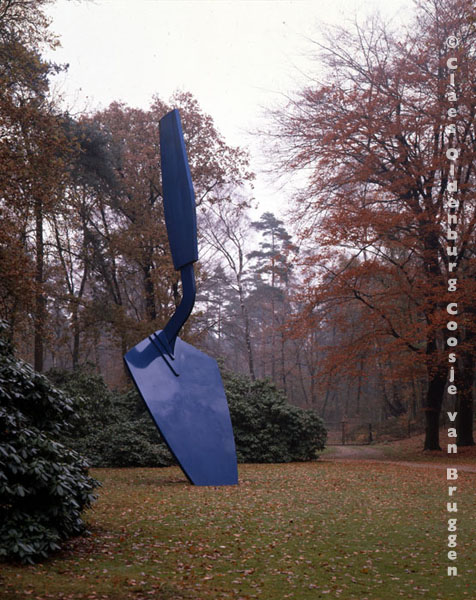
\includegraphics[height=.95\textheight]{trowel.jpeg}
    \centering
    \caption{Trowel I \autocite{pic4}}
    \label{fig:trowel}
\end{figure}

% #endregion Figures ======================

\clearpage
\printbibliography
\end{document}